%	paper.tex	Toby Searle
%	Last modified: Fri  6 Jun 15:39:17 2014
%	using jfm template

\NeedsTeXFormat{LaTeX2e}

\documentclass{jfm}

\usepackage{graphicx}
\usepackage{natbib}
%%%%%%%%%%%Added to template:
\usepackage{caption,subcaption, mathtools} % add my own packages
\graphicspath{ {./images/} }
\newcommand\Wi{\mbox{\textit{Wi}}}
\newcommand{\dt}[1]{\frac{d #1}{d t}} %time deriv
\newcommand{\dy}[1]{\frac{\partial #1}{\partial y}}
%%%%%%%%%%%%%%%

% See if the author has AMS Euler fonts installed: If they have, attempt
% to use the 'upmath' package to provide upright math.
\ifCUPmtlplainloaded \else
  \checkfont{eurm10}
  \iffontfound
    \IfFileExists{upmath.sty}
      {\typeout{^^JFound AMS Euler Roman fonts on the system,
                   using the 'upmath' package.^^J}%
       \usepackage{upmath}}
      {\typeout{^^JFound AMS Euler Roman fonts on the system, but you
                   dont seem to have the}%
       \typeout{'upmath' package installed. JFM.cls can take advantage
                 of these fonts,^^Jif you use 'upmath' package.^^J}%
       \providecommand\upi{\pi}%
      }
  \else
    \providecommand\upi{\pi}%
  \fi
\fi

% See if the author has AMS symbol fonts installed: If they have, attempt
% to use the 'amssymb' package to provide the AMS symbol characters.

\ifCUPmtlplainloaded \else
  \checkfont{msam10}
  \iffontfound
    \IfFileExists{amssymb.sty}
      {\typeout{^^JFound AMS Symbol fonts on the system, using the
                'amssymb' package.^^J}%
       \usepackage{amssymb}%
       \let\le=\leqslant  \let\leq=\leqslant
       \let\ge=\geqslant  \let\geq=\geqslant
      }{}
  \fi
\fi

% See if the author has the AMS 'amsbsy' package installed: If they have,
% use it to provide better bold math support (with \boldsymbol).

\ifCUPmtlplainloaded \else
  \IfFileExists{amsbsy.sty}
    {\typeout{^^JFound the 'amsbsy' package on the system, using it.^^J}%
     \usepackage{amsbsy}}
    {\providecommand\boldsymbol[1]{\mbox{\boldmath $##1$}}}
\fi

%%% Example macros (some are not used in this sample file) %%%

% For units of measure
\newcommand\dynpercm{\nobreak\mbox{$\;$dyn\,cm$^{-1}$}}
\newcommand\cmpermin{\nobreak\mbox{$\;$cm\,min$^{-1}$}}

% Various bold symbols
\providecommand\bnabla{\boldsymbol{\nabla}}
\providecommand\bcdot{\boldsymbol{\cdot}}
\newcommand\biS{\boldsymbol{S}}
\newcommand\etb{\boldsymbol{\eta}}

% For multiletter symbols
\newcommand\Real{\mbox{Re}} % cf plain TeX's \Re and Reynolds number
\newcommand\Imag{\mbox{Im}} % cf plain TeX's \Im
\newcommand\Rey{\mbox{\textit{Re}}}  % Reynolds number
\newcommand\Pran{\mbox{\textit{Pr}}} % Prandtl number, cf TeX's \Pr product
\newcommand\Pen{\mbox{\textit{Pe}}}  % Peclet number
\newcommand\Ai{\mbox{Ai}}            % Airy function
\newcommand\Bi{\mbox{Bi}}            % Airy function

% For sans serif characters:
% The following macros are setup in JFM.cls for sans-serif fonts in text
% and math.  If you use these macros in your article, the required fonts
% will be substitued when you article is typeset by the typesetter.
%
% \textsfi, \mathsfi   : sans-serif slanted
% \textsfb, \mathsfb   : sans-serif bold
% \textsfbi, \mathsfbi : sans-serif bold slanted (doesnt exist in CM fonts)
%
% For san-serif roman use \textsf and \mathsf as normal.
%
\newcommand\ssC{\mathsf{C}}    % for sans serif C
\newcommand\sfsP{\mathsfi{P}}  % for sans serif sloping P
\newcommand\slsQ{\mathsfbi{Q}} % for sans serif bold-sloping Q

% Hat position
\newcommand\hatp{\skew3\hat{p}}      % p with hat
\newcommand\hatR{\skew3\hat{R}}      % R with hat
\newcommand\hatRR{\skew3\hat{\hatR}} % R with 2 hats
\newcommand\doubletildesigma{\skew2\tilde{\skew2\tilde{\Sigma}}}
%       italic Sigma with double tilde

% array strut to make delimiters come out right size both ends
\newsavebox{\astrutbox}
\sbox{\astrutbox}{\rule[-5pt]{0pt}{20pt}}
\newcommand{\astrut}{\usebox{\astrutbox}}

\newcommand\GaPQ{\ensuremath{G_a(P,Q)}}
\newcommand\GsPQ{\ensuremath{G_s(P,Q)}}
\newcommand\p{\ensuremath{\partial}}
\newcommand\tti{\ensuremath{\rightarrow\infty}}
\newcommand\kgd{\ensuremath{k\gamma d}}
\newcommand\shalf{\ensuremath{{\scriptstyle\frac{1}{2}}}}
\newcommand\sh{\ensuremath{^{\shalf}}}
\newcommand\smh{\ensuremath{^{-\shalf}}}
\newcommand\squart{\ensuremath{{\textstyle\frac{1}{4}}}}
\newcommand\thalf{\ensuremath{{\textstyle\frac{1}{2}}}}
\newcommand\Gat{\ensuremath{\widetilde{G_a}}}
\newcommand\ttz{\ensuremath{\rightarrow 0}}
\newcommand\ndq{\ensuremath{\frac{\mbox{$\partial$}}{\mbox{$\partial$} n_q}}}
\newcommand\sumjm{\ensuremath{\sum_{j=1}^{M}}}
\newcommand\pvi{\ensuremath{\int_0^{\infty}%
  \mskip \ifCUPmtlplainloaded -30mu\else -33mu\fi -\quad}}

\newcommand\etal{\mbox{\textit{et al.}}}
\newcommand\etc{etc.\ }
\newcommand\eg{e.g.\ }


\newtheorem{lemma}{Lemma}
\newtheorem{corollary}{Corollary}

\title[Viscoelastic Kelvin-Helmholtz instabilty]{Viscoelastic Kelvin-Helmholtz instability}

\author[T. W. Searle and A. N. Morozov]%
{T. W. Searle$^1$ and A. N. Morozov$^1$%
  \thanks{Email address for correspondence: jfm@damtp.cam.ac.uk},\ns
}

% NOTE: A full address must be provided: department, university/institution, town/city, zipcode/postcode, country.
\affiliation{$^1$SUPA, School of Physics and Astronomy, University of Edinburgh, Mayfield Road,
Edinburgh, EH9 3JZ, UK\\[\affilskip]
}

\pubyear{2013}
\volume{650}
\pagerange{119--126}
% Do not enter received and revised dates. These will be entered by the editorial office.
\date{?; revised ?; accepted ?. - To be entered by editorial office}
%\setcounter{page}{1}
\begin{document}

\maketitle

\begin{abstract}
  Abstract goes here. Abstract goes here. Viscoelastic Kelvin-Helmholtz instability. 
\end{abstract}

\begin{keywords}
Authors should not enter keywords on the manuscript, as these must be chosen by
the author during the online submission process and will then be added during
the typesetting process (see
http://journals.cambridge.org/data/\linebreak[3]relatedlink/jfm-\linebreak[3]keywords.pdf
for the full list)
\end{keywords}

\section{Introduction}

Turbulence without inertia in viscoelastic fluids has generated much interest
since it was discovered in Taylor-Couette flow by Larson, Shaqfeh and Muller in
1990 \cite{Larson1990}. As well as this numerical and experimental study of
Taylor-Couette flow, Groisman and Steinberg \cite{Groisman2000} discovered
turbulence in viscoelastic fluids between two counter rotating plates.

It was long thought that the elasticity of a viscoelastic fluid only served to
dampen instability. This view stems from early results showing that drag in a
turbulent Newtonian flow can be reduced by the addition of small amounts of
viscoelastic fluid (\cite{Toms1977}). Although drag reduction has received a
lot of attention in the past, studies on turbulence without inertia give reason
to believe that there may be purely elastic instabilities present in elastic
fluids relevent to industry.  This purely elastic turbulence is present at very
low Reynolds number, where it is driven by the elasticity of the polymeric
fluid rather than its inertia.

In 1997 Fabian Waleffe identified a Newtonian self sustaining process in plane
Couette flow \cite{Waleffe1997}. Streamwise rolls redistribute the streamwise
velocity into a streaky flow. This streaky flow is unstable through a
Kelvin-Helmholtz instability leading to a symmetry bifurcation to a three
dimensional flow. Finally, the nonlinear effects due to this instability
re-energises the original streamwise rolls. This exact solution to the
Navier-Stokes equations is thought to be a component of the transition to
turbulence. In 1998 Waleffe constructed a bifurcation diagram for this exact
solution \cite{Waleffe1998} containing what looks like a bifurcation from
infinity, just the behaviour expected of the transition to turbulence in plane
Couette flow.

Using this work in Newtonian fluid dynamics as a template for the structure of
purely elastic turbulence reveals a similar pattern of streaks and, hopefully,
a similar self-sustaining process \cite{US!}. An important step towards
explaining this process in purely elastic flows is establishing the mechanism
by which the streaks become unstable. Presumably, this will also be a
Kelvin-Helmholtz instability as the streaks shear with the rest of the fluid.
The Kelvin-Helmholtz instability is also often integral to the transition to
turbulence in Newtonian fluids. It is hoped that by finding a purely elastic
version of this instability, we might be able to probe one of the important
mechanisms for the transition to purely elastic turbulence. To explore this
mechanism in the purely elastic regime we have constructed a simple model
system of a shearing viscoelastic fluid.

The key dimensionless number for turbulence without inertia in viscoelastic
flows is the Weissenberg number, which is the ratio of the normal stress to the
shear stress of the polymer component of the fluid $Wi = \frac{N_{1}}{\sigma} =
\lambda \dot{\gamma}$ where $\dot{\gamma}$ is the shear rate.

We present a linear stability analysis of the Kelvin-Helmholtz instability in
the purely elastic regime using direct numerical simulation of both the
Oldroyd-B and FENE-P constitutive models for a polymeric fluid. The purely
elastic fluid is found to be unstable at sufficiently high numbers of the
dimensionless parameter, the Weissenberg number. The growth rate of the largest
growing eigenmode of the instability is found to increase with increasing
Weissenberg number for low Reynold's number. This behaviour is consistent
across both the Oldroyd-B and FENE-P models.

The system we use for our analysis uses a hyperbolic tangent shaped laminar
profile for the streamwise velocity across a channel, where the instability
takes place between $y = \pm \Delta$. $y=0$ is the centreline of the channel,
so that if $\Delta << 1$ the flow can be said to be a free shear instability.
This gives a base flow profile, 
\begin{align}
    U(y) &= \tanh \left( y/\Delta \right) \coth \left( 1/\Delta \right) \nonumber\\
    V &= 0 \nonumber \\
    T_{xx}(y) &= 2 Wi \left( \dy{U} \right)^{2} \nonumber \\
    T_{xy}(y) &= \dy{U} \nonumber \\
    T_{yy}(y) &= 0 \nonumber 
    \label{eq:KH_laminar_profile}
\end{align}

$U$ and $V$ are the base streamwise (x) and wall normal (y) velocities
respectively. $T$ is the base stress tensor. We use Gauss-Labatto points in the
wall-normal ($y$) direction for the base profile, and decomposed the
disturbances to this flow into Fourier modes.  
\begin{equation}
    g(y) = \sum\limits_{n=-N}^{N} \widetilde{g}(y) e^{ikx + \lambda t}
\end{equation}
for all disturbance variables $g = u, v, p, \tau_{i,j}$. Where $N$ is the
number of Fourier modes, $k$ is the streamwise wavenumber of the disturbance
and $\lambda$ is the growth rate of the mode. This program uses two domains of
pseudo-spectral points to give increased resolution in the centre of the
simulation. The simulation was also repeated using a code for which the system
of points was stretched using: 
\begin{align}
    z_{u} &= \frac{y_{u}}{1-y_{u}} \\
    z_{b} &= \frac{y_{b}}{1+y_{b}} \\
    U     &= \tanh{z/\Delta} 
    \label{eq:KH_inf_profile}
\end{align}
This system ought to be completely insensitive to the boundary conditions on
the flow and so also behave as a free shear instability. 

The dimensionless quantities used throughout are non-dimensionalised relative
to the instability size, $\Delta$, rather than the total simulation size. The
obvious reason for this is that $\Delta$ is the length scale for the free shear
instability.

In order to simulate this flow, we used an Oldroyd-B fluid with very low
Reynolds number $\Rey < 0.01$ and a small ratio between the solvent and total
viscosities $\beta = \frac{\mu_{s}}{\mu_{s}+\mu_{p}}$. This approximates a
purely elastic fluid, where the polymer contribution to the dynamics is higher
than the solvent contribution. The Oldroyd-B Navier stokes and constitutive
equations are then: 
\begin{align}
    Re \left[ \dt{\mathbf{v}} + \mathbf{v} \cdot \nabla  \mathbf{v} \right] &=
    - \nabla p + \beta \nabla^{2} \mathbf{v} + \frac{1-\beta}{Wi} \nabla \cdot
    \mathbf{\tau} \\ \dot{\tau}/Wi + \overset{\nabla}\tau &= \left(\nabla
    \mathbf{v}\right)^{T} + \nabla{\mathbf{v}}
\end{align}
With $\mathbf{v}$ as the total (base flow and disturbance) velocity and $\tau$
as the total stress in the polymeric fluid. The FENE-P viscoelastic fluid has
the advantage of being similarly easy to simulate, but also including a finite
extensibility for the polymers. This leads to a stress which depends on a
conformation tensor ($\mathbf{C}$) for the polymer dumbbells via a non-linear
spring force:

\begin{equation}
    \mathbf{\tau} = \frac{1-\frac{3}{L^{2}}}{1 + \frac{L^{2}}{tr(\mathbf{C^{2}})}}
\end {equation}

\begin{figure}
    \centering
    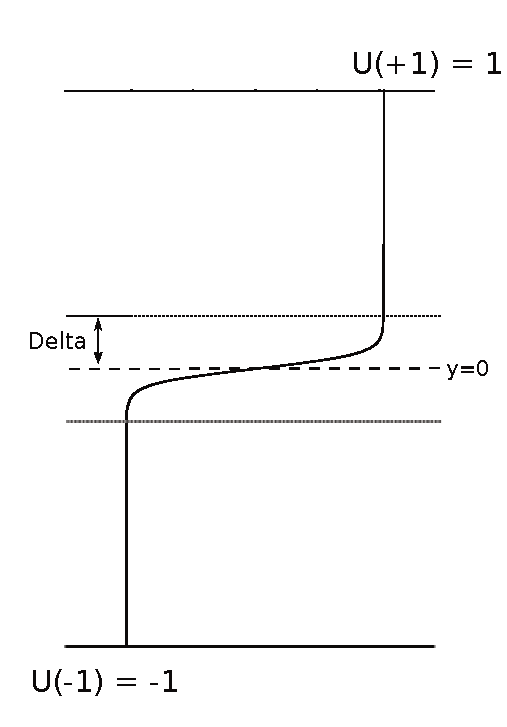
\includegraphics[width=0.3\textwidth]{KH_diagram}
    \caption{diagram of the system}
    \label{fig:diagram}
\end{figure}

Again, we used Gauss-Labatto points in the wall normal direction and Fourier
modes in the streamwise direction.

\section{A purely elastic instability}

At low Reynolds number, low $\beta$ and sufficiently large Weissenberg number
we observe an instability across a range of streamwise disturbance wavenumbers.
This leads us to suppose that this instability might be a plausible cause for a
self-sustaining process in viscoelastic plane Couette flow, similar to that
observed by Waleffe.

The instability remains unchanged under variation of $\Delta$ at low $\Delta$,
proving that it is a free shear instability. Although the instability appears
to require some inertia in the fluid, it is still present for  $\Rey = 0.01$,
far lower than the usual threshold of $\Rey = 1000$ for a Newtonian
Kelvin-Helmholtz instability.

We see an instability grow from around $k \sim 0.06$ and move to lower $k$ as
the Weissenberg number increases (figure \ref{fig:dispersions_low_Re}). The
height of the instability also increases with increasing Weissenberg number
(figure \ref{fig:inf_low_Re}). 

\begin{figure}
    \centering
    \begin{subfigure}[b]{0.48\textwidth}
	\centering
	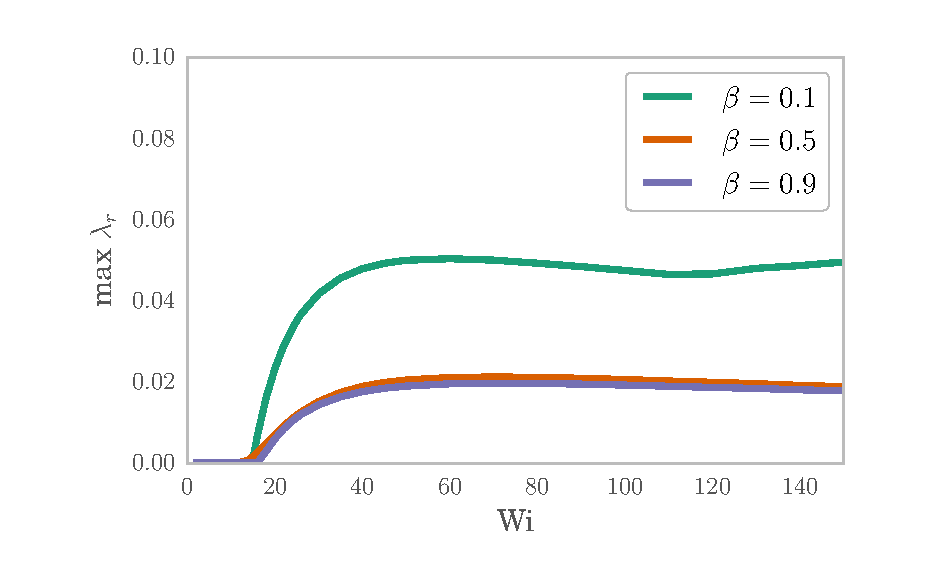
\includegraphics[width=\textwidth]{inf_purely_elastic}
	\caption{}
	\label{fig:inf_low_Re}
    \end{subfigure}
    ~
    \begin{subfigure}[b]{0.48\textwidth}
	\centering
	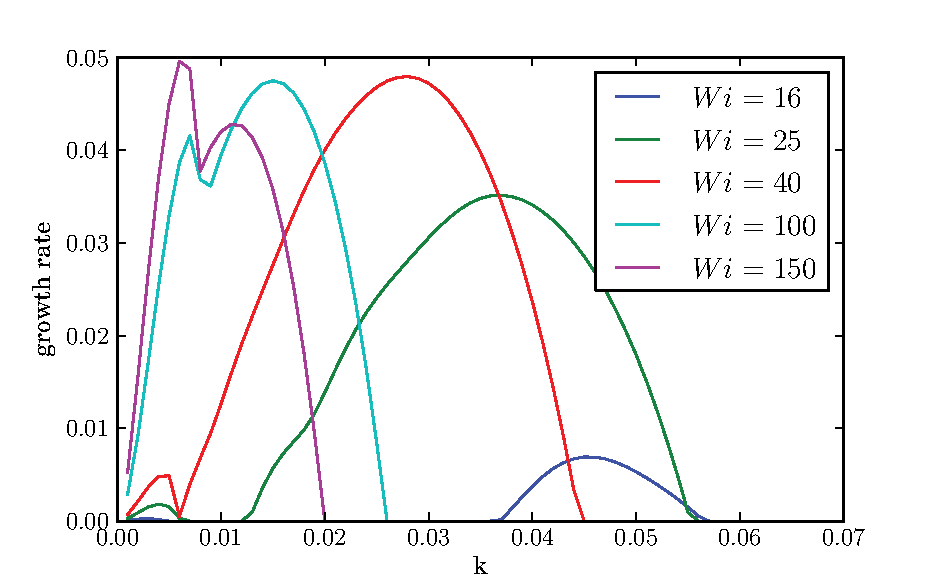
\includegraphics[width=\textwidth]{inf_dispersions_low_Re}
	\caption{}
	\label{fig:dispersions_low_Re}
    \end{subfigure}
    \caption{a) Free shear version of the instability. Plot of the maximum
	     growth rate against Wiessenberg number at $\Rey = 0.01$. b)
	     Dispersion relations at various Weissenberg numbers to accompany
	     the trend in figure a).}
\end{figure}

The dispersion relation saturates at $Wi \sim 50$ and remains approximately
constant with increasing Weissenberg number. The dispersion relation for the
instability remains broad in $k$ until $Wi \sim 100$ where a new eigenvector
becomes dominant.

\begin{figure}
    \centering
    \begin{subfigure}[b]{0.48\textwidth}
	\centering
	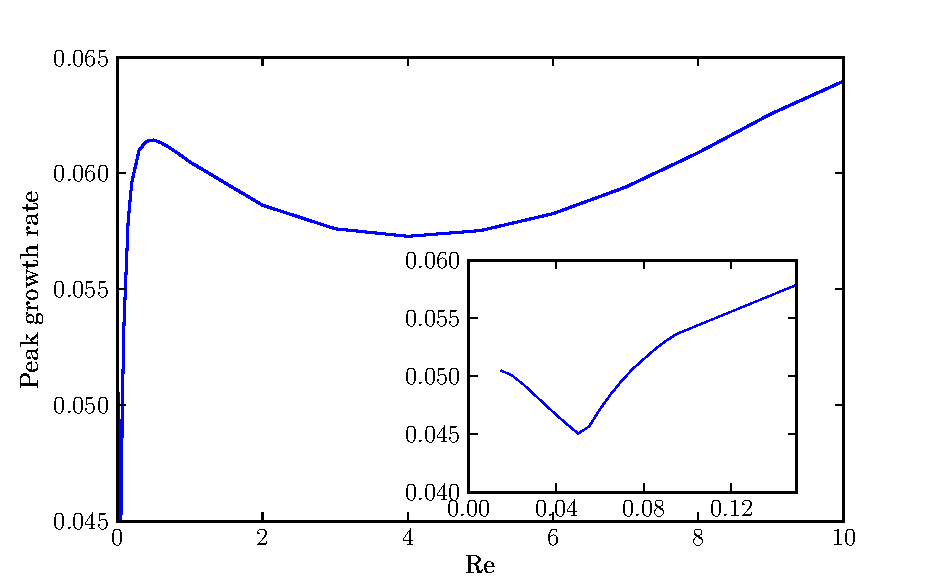
\includegraphics[width=\textwidth]{inf_vary_Re}
	\caption{}
	\label{fig:inf_vary_Re}
    \end{subfigure}
    ~
    \begin{subfigure}[b]{0.48\textwidth}
	\centering
	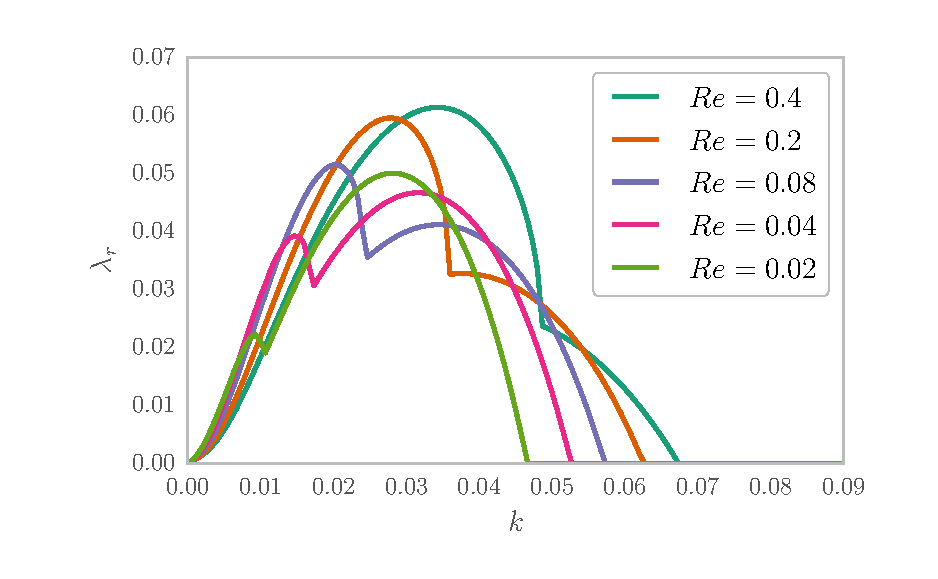
\includegraphics[width=\textwidth]{inf_dispersions_low_Wi}
	\caption{}
	\label{fig:dispersions_low_Wi}
    \end{subfigure}
    \caption{
	a) Free shear version of the instability. Plot of the maximum growth
	rate against Reynold's number with $\Wi=50$. b) Dispersion relations at
	various Reynold's numbers to accompany the trend in figure a).
    } 
    \end{figure}

As the Reynold's number is reduced, new eigenvalues become dominant. Although
the dominant eigenvalue changes the flow is still unstable, even down to $\Rey
= 0.01$ (see figures \ref{fig:inf_vary_Re} and \ref{fig:dispersions_low_Wi}).


\subsection{ Shear instability with walls}

If we examine the eigenvectors of the instability, we see that there are very
large polymer stresses in the $\pm \Delta$ region. This corresponds to the
large shear rate brought about as the two flows pass each other. Examining the
flow field, we see that there are large vortices arranged with opposite
rotational directions above and below the shear region which extend almost to
the walls. 

\begin{figure}
    \begin{subfigure}[b]{\textwidth}
    \centering
    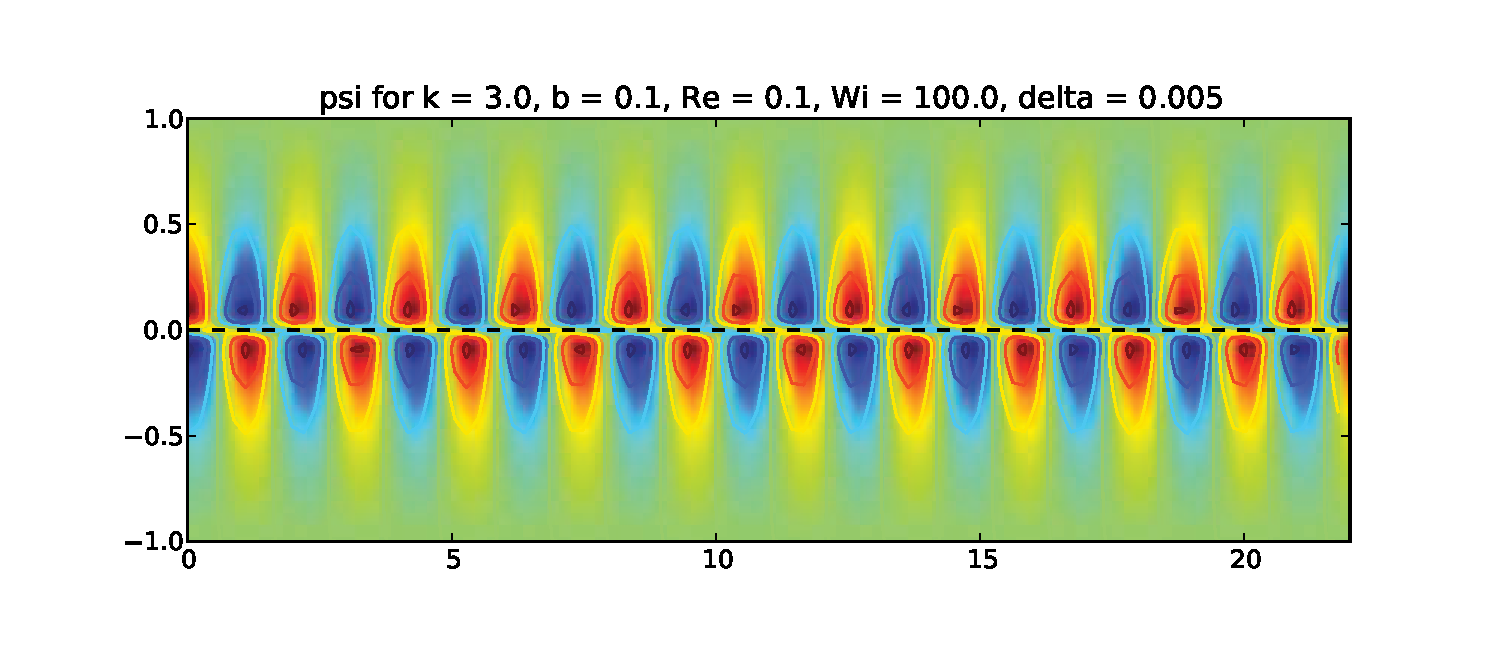
\includegraphics[width=\textwidth]{psi_low_delta}
    \caption{}
    \label{fig:psi_low_delta}
    \end{subfigure}
    \vspace{1 mm}
    \begin{subfigure}[b]{\textwidth}
    \centering
    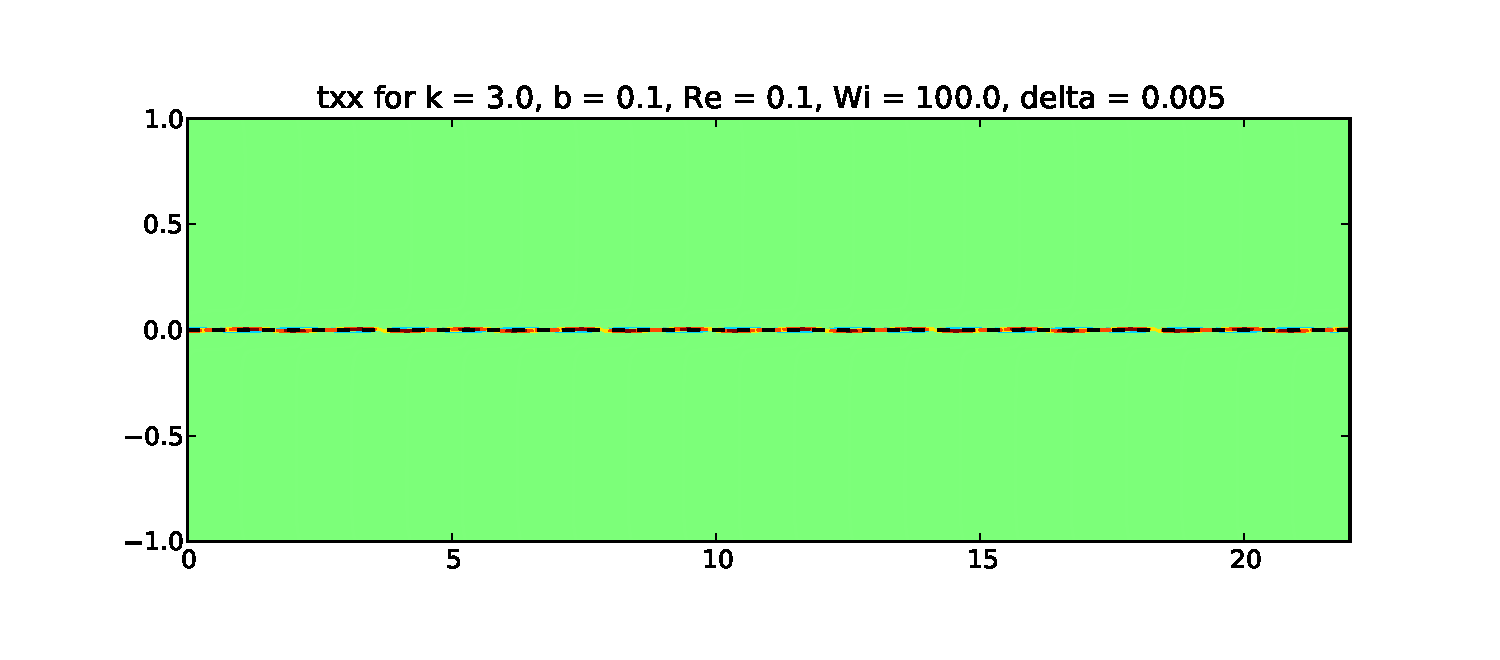
\includegraphics[width=\textwidth]{txx_low_delta}
    \caption{}
    \label{fig:stress_low_delta}
    \end{subfigure}
    \caption{
	a) Streamfunction of the largest eigenfunction of the instability when
	$\Rey = 0.1$, $\Wi =100$, $\Delta = 0.005$. Red is positive
	(streamlines of the flow point clockwise around the contours), Blue is
	negative (streamlines of the flow point anticlockwise around the
	contours) b) xx stress for the same instability.
    }
\end{figure}

Dependence of the instability on the channel walls persists at very small
$\Delta$. We believe that this is due to the inertial effects at low Reynold's
number being so weak. This means it is very easy to move the fluid even at
the shear rate present far from the centre of the channel. I think the
instability generated by the elasticity of the fluid needs the walls to dampen
it for some reason. 

\begin{figure}
    \centering
    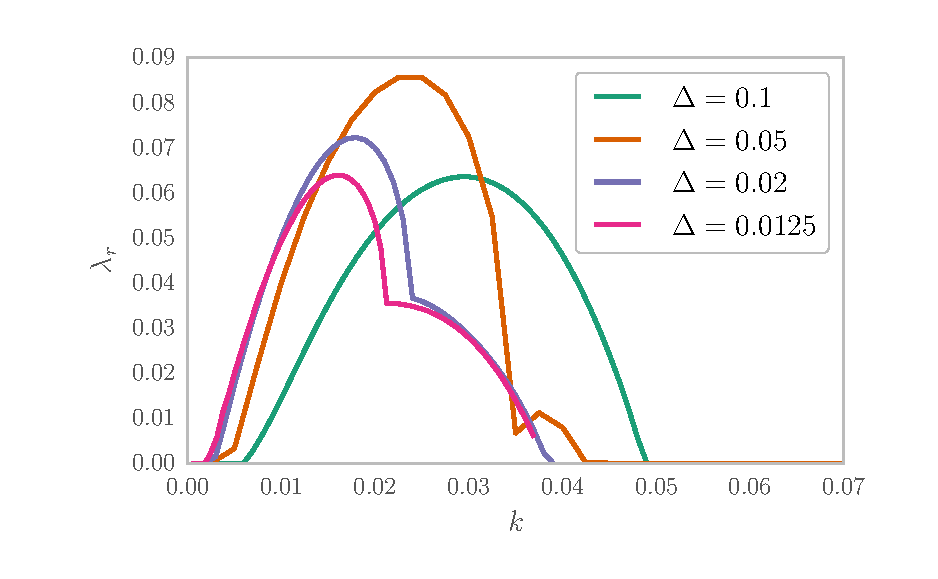
\includegraphics[width=\textwidth]{KH_vary_delta}
    \caption{
    Dispersion relations for various values of $\Delta$ at $\Rey = 0.1$, $\Wi =
    100$. The sensitivity to the walls seems only to increase the strength of
    the instability. Even when the system is insensitive to the walls, at
    $\Delta= 0.0125$, there is still an instability present.
    }
    \label{fig:walls_dependence}
\end{figure}

\begin{figure}
    \centering
    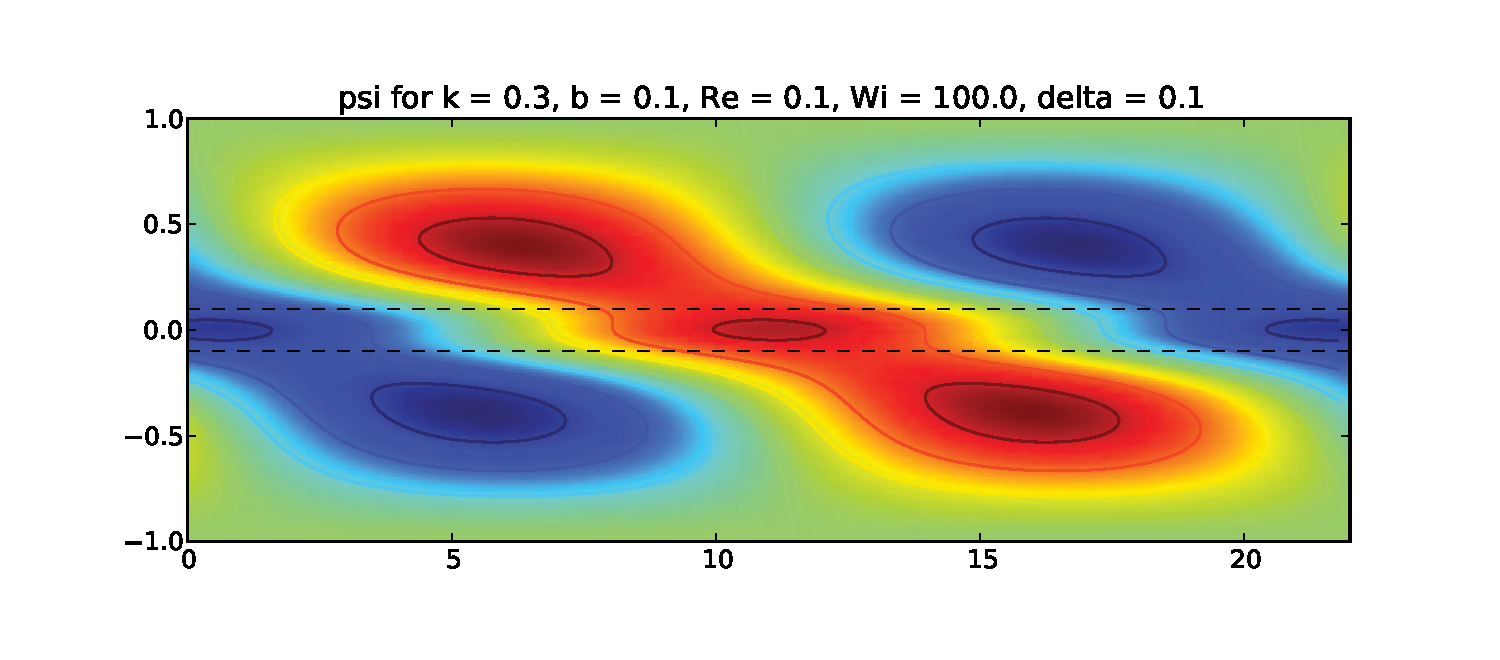
\includegraphics[width=\textwidth]{psi_high_delta}
    \caption{
    Streamfunction of the eigenfunction of the instability at $\Delta = 0.1$,
    $\Wi = 100$, $\Rey=0.1$. The magnitude is scaled by the xx stress in the
    centre of the channel.
    }
    \label{fig:psi_high_delta}
\end{figure}

It is difficult to see the instability at $\Rey = 0$. As the Reynold's number
is reduced the walls become more important to the instability. In order to
remove the dependence on the walls and recover a free shear instability it is
necessary to move them further away. This problem gets worse at lower $\Rey$.
By introducing just a very small contribution from inertia, we can remove the
dependence on the walls. This is why all of our results are taken for $\Rey
\leq 0.1$ on the length scale of the instability.

The reason we have have the simulation with the walls at all is because of the
implications for the plane Couette problem. The Kelvin-Helmholtz instability in
the Newtonian problem takes place on a length scale of about 10\% of the width
of the channel, or $\Delta = 0.1$ (a guess). The viscoelastic Kelvin-Helmholtz
instability is sensitive to the walls at this $\Delta$ and a $\Rey \lesssim 1$
(see figure \ref{fig:vary_Re_delta_conv}). This means that on the scale of the
channel, $\Rey \gtrsim 10$ for the walls not to affect the instability. So, the
important results for the purely elastic instability from the point of view of
the plane Couette problem are probably those for which the walls are relevant. 

\begin{figure}
    \centering
    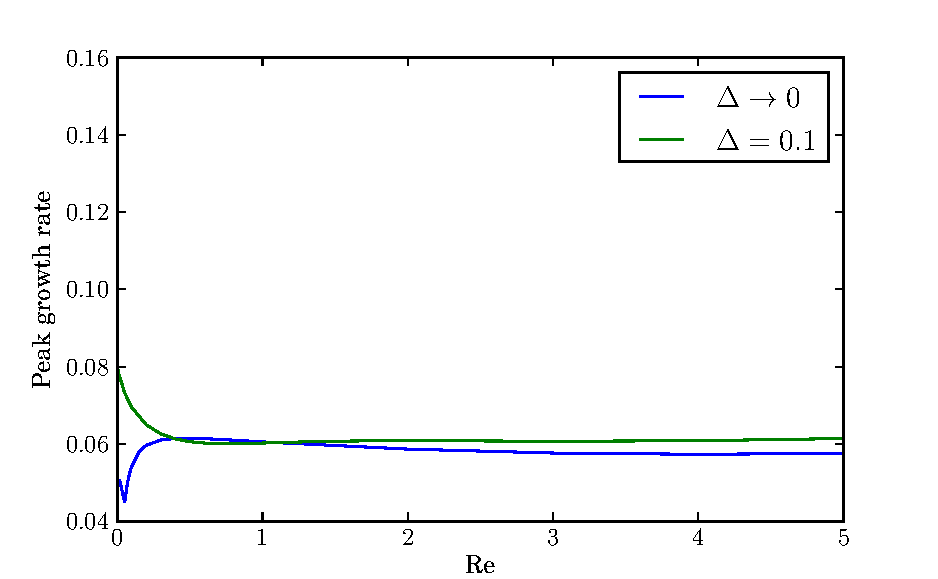
\includegraphics[width=0.7\textwidth]{vary_Re_delta_conv}
    \caption{
	The blue line is the data from the stretched code and the green line is
	the $\Delta = 0.1$ data. By $\Rey = 1$ it is clear that the Reynold's
	number is sufficient such that the walled system behaves as though it
	were insensitive to the walls.
    }
    \label{fig:vary_Re_delta_conv}
\end{figure}

At $\Delta = 0.1$ we see the same instability as that seen in the completely
free case. 

\begin{figure}
    \centering
    \begin{subfigure}[b]{0.48\textwidth}
	\centering
	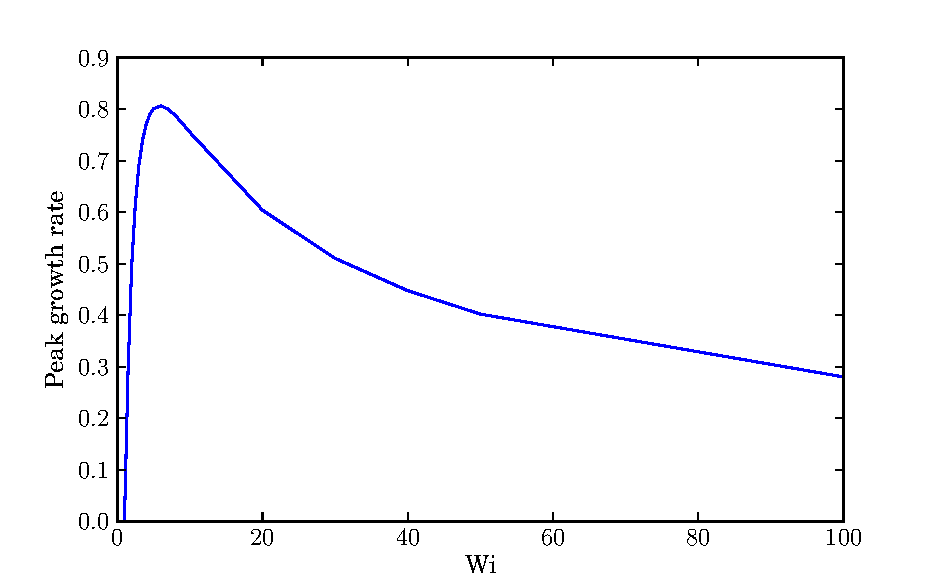
\includegraphics[width=\textwidth]{KH_purely_elastic}
    \caption{}
    \label{fig:KH_purely_elastic}
\end{subfigure}
~
\begin{subfigure}[b]{0.48\textwidth}
    \centering
    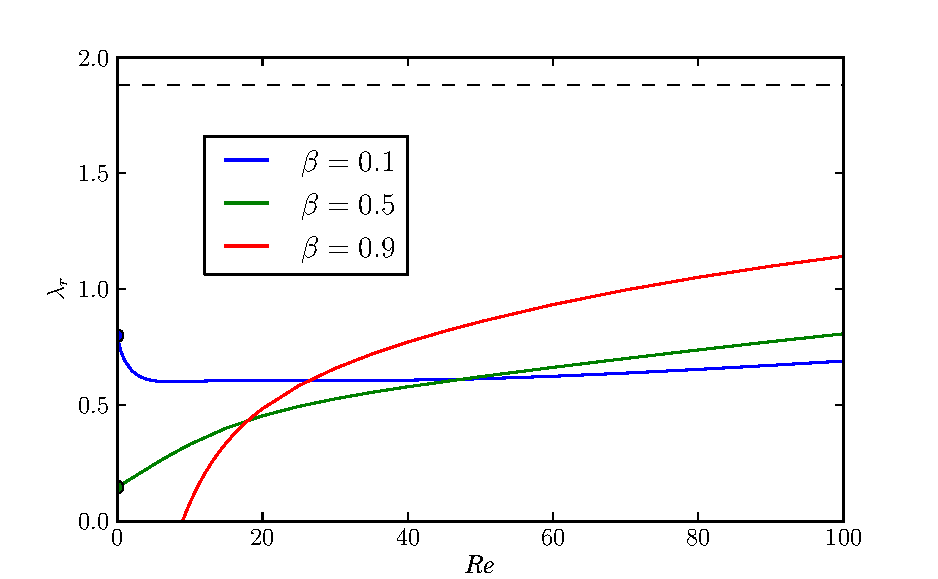
\includegraphics[width=\textwidth]{KH_low_Wi_vary_Re}
    \caption{}
    \label{fig:KH_reduce_Re}
\end{subfigure}

\begin{subfigure}[b]{0.48\textwidth}
    \centering
    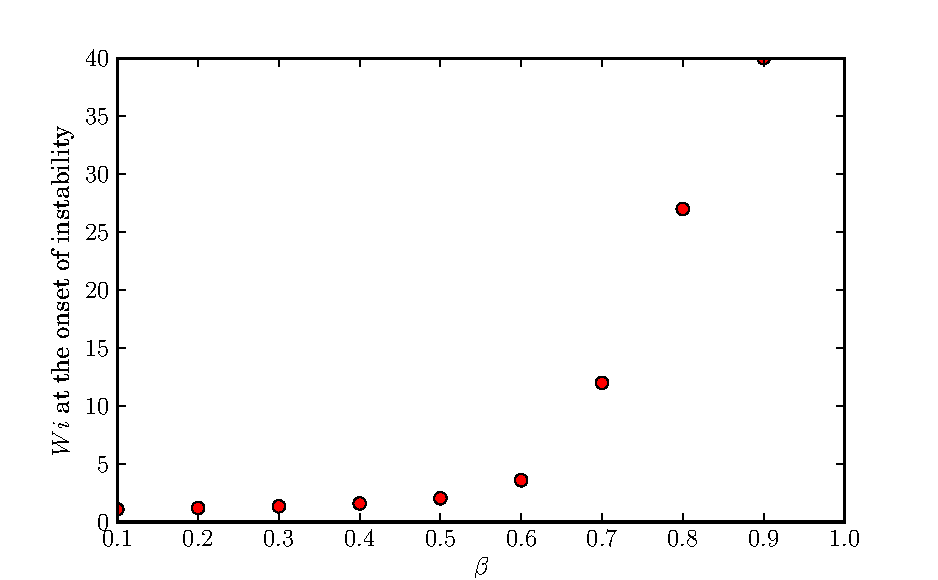
\includegraphics[width=\textwidth]{KH_onset_beta_Wi}
    \caption{}
    \label{fig:KH_elastic_onset}
\end{subfigure}
~
\begin{subfigure}[b]{0.48\textwidth}
    \centering
    \includegraphics[width=\textwidth]{fin_dispersions_Wi50}
    \caption{}
    \label{fig:KH_finite_dispersions}
\end{subfigure}
\caption{
a) The change in the height of the dispersion relation as $\Wi$ is increased at
$\Rey = 0$ with $\Delta = 0.1$. This instability must be entirely elastic in
nature. b) The change in the height of the dispersion relation as the Reynolds
number is reduced at $\Wi=5$. At low $\Rey$ the instability is clearly still
present for large polymer concentrations, consistent with purely elastic
turbulence with $\Delta = 0.1$.  c) The value of the Weissenberg number at
which the velocity profile becomes unstable against $\beta$ at $\Delta = 0.1$.
The onset of the purely elastic instability moves to higher $Wi$ as $\beta$
increases. d) Dispersion relations at Wi =50 for $\Delta =0.1$.
}
\end{figure}

\section{Confirming the model}

\subsection{Consistency of results with the FENE model}

The finite extensibility version of the model gives good agreement with the
Oldroyd-B version. Shorter lengths bring about a larger instability but do not
delay it to higher Weissenberg number. Otherwise similar dispersion relations
are observed with a similar dependence on the distance to the walls (figure
\ref{fig:FENE_low_Re}).

\begin{figure}
    \centering
    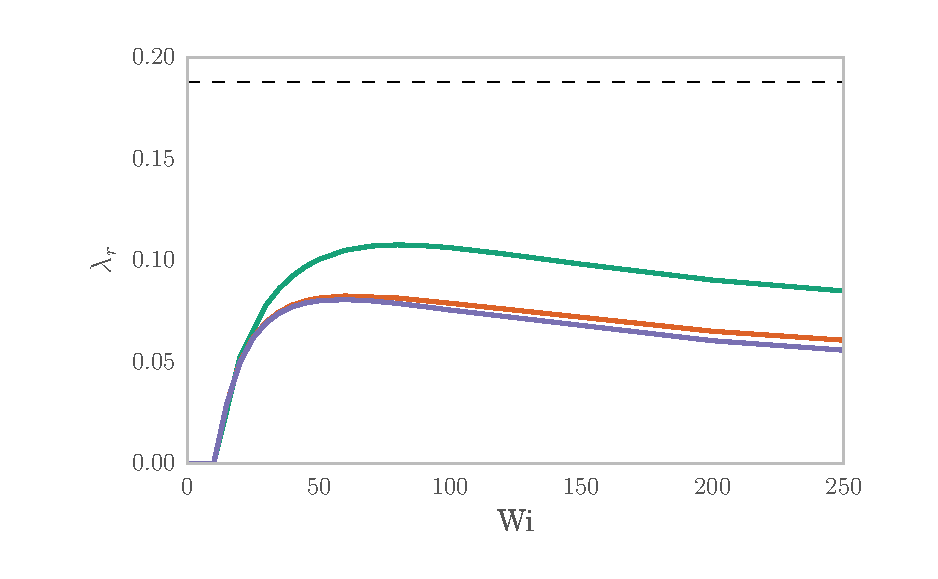
\includegraphics[width=0.7\textwidth]{FENE_purely_elastic}
    \caption{
    The FENE-P model fluid at $\Rey = 0$  when $\Delta = 0.1$. Results are
    consistent with figure \ref{fig:KH_purely_elastic}.
    }
    \label{fig:FENE_low_Re}
\end{figure}

\subsection{Varying width of the instability}

\begin{figure}
    \centering
    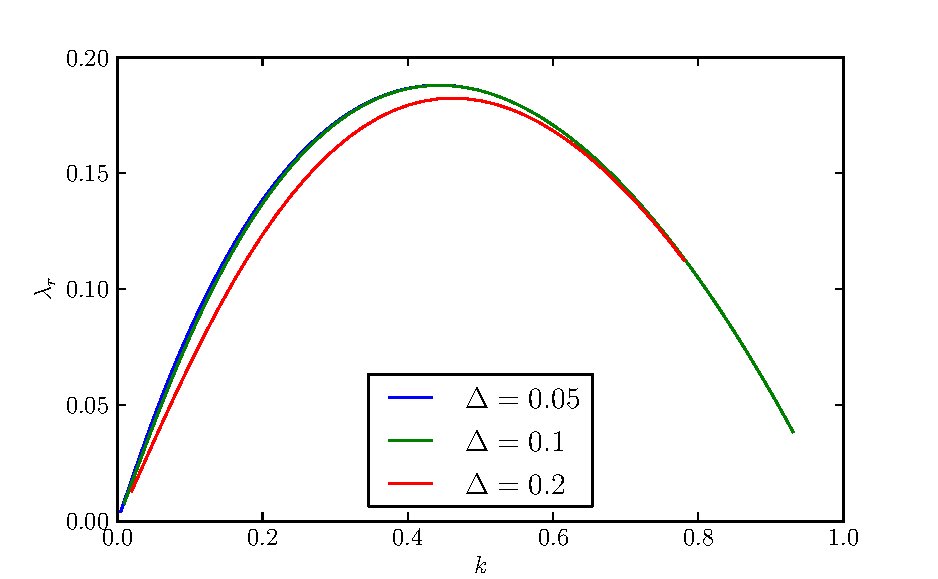
\includegraphics[width=0.7\textwidth]{high_Re_vary_delta}
    \caption{ 
    Dispersion relations for various values of $\Delta$ and $\Rey = 1000$, $\Wi
    = 0.01$. When results are rescaled for delta, The instability is found to
    be insensitive to the width of the instability relative to the wall at this
    combination of Reynold's number and Wiessenberg number.
    }
    \label{fig:delta_dispersion}
\end{figure}


\subsection{Drag reduction}

We see drag reduction using the Oldroyd-B model. It is not clear whether or not
the maximum drag reduction asymptote is present (figure
\ref{fig:KH_drag_reduction}).



\begin{figure}
%    \showthe\columnwidth %use this to determine size of figures.
    \centering
    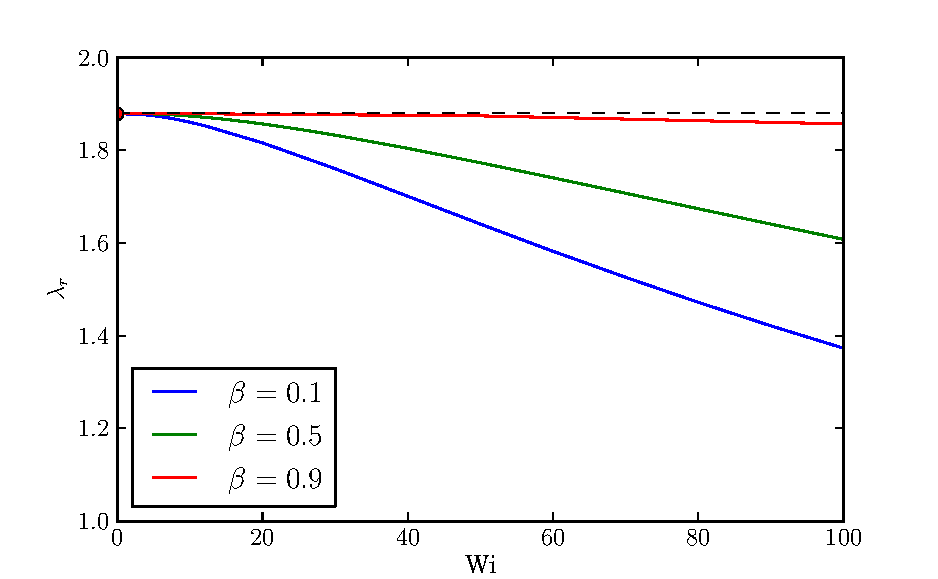
\includegraphics[width=0.7\textwidth]{KH_high_Re_vary_Wi}
    \caption{
	Peak growth rate against Wiessenberg number at $\Rey = 1000$, $\Delta =
	0.1$ The height of the dispersion relation is reduced for the
	Kelvin-Helmholtz instability as the Weissenberg number is increased.
	The grey dashed line is the height of the dispersion relation for the
	Newtonian fluid. The decrease in $\lambda_{r}$ corresponds to increased
	stability of the base flow and so confirms the presence of drag
	reduction in this system.
    }
    \label{fig:KH_drag_reduction}
\end{figure}

\section{Outline of the mechanism}

\section{Conclusions}

In conclusion, we can say that there is a Kelvin-Helmholtz like instability for
purely elastic shear flows. The unstable region is much larger than that seen
in Newtonian fluids relative to the region of shear. The wavenumber of the
instability is much smaller in the viscoelastic case ($k<0.06$), suggesting a
larger minimal flow unit is required in viscoelastic fluids. This instability
is enhanced slightly by introducing a finite extensibility to the polymers but
remains of essentially the same form. The instability has grown to its maximum
by the time it reaches an effective Weissenberg number $ Wi \sim 50$ after
which it is saturated. The instability is also strongly dependent on the walls
at low effective Reynold's number.

\bibliographystyle{jfm}
% Note the spaces between the initials


\bibliography{KH_paper}

\end{document}
